\documentclass[10pt,aspectratio=169]{beamer}

% All the boilerplate is in raslides.sty
% Note that this also pulls in a custom vogtwidebar.sty
\usepackage{raslides}

\author{Ji\v{r}\'i Lebl}

\institute[OSU]{%
Departemento pri Matematiko de Oklahoma {\^S}tata Universitato}

\title{BA: 3.1}

\date{}

\begin{document}

\begin{frame}
\titlepage
\end{frame}

\begin{frame}
\begin{definition}
Let $S \subset \R$ be a set.  A number $x \in \R$ is called
a \emph{cluster point} of $S$
if for every $\epsilon > 0$, the set $(x-\epsilon,x+\epsilon) \cap S
\setminus \{ x \}$ is not empty.
\end{definition}

\pause

I.e.,
$x \in \R$ is a cluster point of $S$ if $\forall$ $\epsilon > 0$ ~$\exists$ $y \in
S$ s.t. $y \not= x$ and $\abs{x - y} < \epsilon$.

\pause
\medskip

Note: A cluster point of $S$ need not lie in $S$.

\pause
\medskip

\textbf{Examples:}
\begin{enumerate}[(i)]
\item
$\{ \nicefrac{1}{n} : n \in \N \}$ has a unique cluster point: $0$.
\item\pause The set of cluster points of $(0,1)$ is
$[0,1]$.
\item\pause
The set of cluster points of $\Q$ is $\R$.
\item\pause
The set of cluster points of $[0,1) \cup \{ 2 \}$ is $[0,1]$.
\item\pause
$\N$ has no cluster points.
\end{enumerate}

\end{frame}

\begin{frame}

\begin{proposition}
Let $S \subset \R$.  Then $x \in \R$ is a cluster point of $S$
if and only if
there exists a convergent sequence of numbers $\{ x_n \}_{n=1}^\infty$ such that
$x_n \not= x$ and $x_n \in S$ for all $n$, and $\lim\limits_{n\to\infty} x_n = x$.
\end{proposition}

\pause
\textbf{Proof:}
Suppose $x$ is a cluster point of $S$.

\pause
%\medskip

For every $n \in \N$, pick $x_n$ to be an arbitrary point of
$(x-\nicefrac{1}{n},x+\nicefrac{1}{n}) \cap S \setminus \{x\}$.

($x_n$ exists as $x$ is a cluster point of $S$).

\pause
%\medskip

$x_n$ is within $\nicefrac{1}{n}$ of $x$: \quad
$\abs{x-x_n} < \nicefrac{1}{n}$.


\pause
%\medskip

$\{ \nicefrac{1}{n} \}_{n=1}^\infty$ converges to zero,
$\{ x_n \}_{n=1}^\infty$ converges to $x$.

\pause
\medskip

On the other hand, 

suppose $\{ x_n \}_{n=1}^\infty$ is a seq. in $S \setminus \{ x \}$ converging to $x$.

\pause
\thus \quad
for every $\epsilon > 0$ ~ $\exists$ $M$ such that $\abs{x_M - x} < \epsilon$.

\pause
\thus \quad $x_M \in (x-\epsilon,x+\epsilon) \cap S \setminus \{x\}$.
\qed

\end{frame}

\begin{frame}

\begin{definition}
Consider $f \colon S \to \R$ where $c$ is a cluster point of $S \subset \R$.

\pause
\medskip

Suppose $\exists$ $L \in \R$ and $\forall$ $\epsilon > 0$,
$\exists$ $\delta > 0$ such that whenever $x \in S \setminus \{ c \}$
and $\abs{x - c} < \delta$, we have
\quad
$\abs{f(x) - L} < \epsilon$.

\pause
\medskip

We then say $f(x)$ \emph{converges} to $L$ as $x$ goes
to $c$.

\pause
We say $L$ is the \emph{limit} of $f(x)$ as $x$ goes to $c$.

\pause
\medskip

We write \quad
$\displaystyle
\lim_{x \to c} f(x) \coloneqq L$, \quad
or \quad
$f(x) \to L$ ~as~ $x \to c$.

\pause
\medskip

If no such $L$ exists, we say the limit does not exist or
that $f$ \emph{diverges} at $c$.
\end{definition}

\pause
\textbf{Cheating again:} The notation assumes the limit is unique,

we'll prove that momentarily.

\pause
\medskip

\textbf{Remark:} It is irrelevant whether $f(c)$ is defined or not.

\pause
The limit may not equal $f(c)$, even if $f(c)$ is defined.
\end{frame}

\begin{frame}

\begin{proposition}
Let $c$ be a cluster point of $S \subset \R$ and let $f \colon S \to \R$
be such that $f(x)$ converges as $x$ goes to $c$.
\pause
Then the limit of $f(x)$ as $x$ goes to $c$ is unique.
\end{proposition}

\pause
\textbf{Proof:}
Let both $L_1$ and $L_2$ satisfy the definition.

\pause
Let $\epsilon > 0$ be given.

\pause
Find $\delta_1 > 0$ such that $\abs{f(x)-L_1} < \nicefrac{\epsilon}{2}$ 
for all $x \in S \setminus \{c\}$ with $\abs{x-c} < \delta_1$.

\pause
Find $\delta_2 > 0$ such that $\abs{f(x)-L_2} < \nicefrac{\epsilon}{2}$
for all $x \in S \setminus \{c\}$ with $\abs{x-c} < \delta_2$.

\pause
Put $\delta \coloneqq \min \{ \delta_1, \delta_2 \}$.

\pause
Suppose $x \in S$, $\abs{x-c} < \delta$, and $x \not= c$.

(such an $x$ exists as $c$ is a cluster point).

\pause
\medskip

$\displaystyle
\abs{L_1 - L_2}
\pause
=
\abs{L_1 - f(x) + f(x) - L_2}
\pause
\leq
\abs{L_1 - f(x)} + \abs{f(x) - L_2}
\pause
<
\frac{\epsilon}{2} + \frac{\epsilon}{2}
= \epsilon$.

\pause
\medskip

\thus \quad $L_1 = L_2$.
\qed
\end{frame}

\begin{frame}

\textbf{Example:}
Consider $f \colon \R \to \R$ given by $f(x) \coloneqq x^2$.  Then
for any $c \in \R$,
\begin{equation*}
\lim_{x\to c} f(x) = \lim_{x\to c} x^2 = c^2 .
\end{equation*}

\pause
\textbf{Proof:} Fix $c \in \R$, and let $\epsilon > 0$ is given.

\pause
Let $\delta \coloneqq \min \left\{ 1 , \, \dfrac{\epsilon}{2\abs{c}+1} \right\}$.

\pause
Take $x \not= c$ such that $\abs{x-c} < \delta$ (in particular, $\abs{x-c} < 1$).

\pause
By reverse triangle inequality,
\quad
$\abs{x}-\abs{c} \leq \abs{x-c} < 1$.

\pause
\thus \quad $\abs{x} + \abs{c} < 2\abs{c} + 1$.

\pause
\medskip

Then

\medskip

$\abs{f(x) - c^2}
\pause
= \abs{x^2-c^2}
\pause
= \abs{(x+c)(x-c)}
\pause
= \abs{x+c}\abs{x-c}
$

\pause
\medskip

\qquad\qquad\,\!
$
\leq (\abs{x}+\abs{c})\abs{x-c}
\pause
< (2\abs{c}+1)\abs{x-c}
\pause
< (2\abs{c}+1)\dfrac{\epsilon}{2\abs{c}+1} = \epsilon$. \qed

\end{frame}

\begin{frame}

\textbf{Example:}
Define $f \colon [0,1) \to \R$ by
\quad
$\displaystyle
f(x) \coloneqq 
\begin{cases}
x & \text{if } x > 0 , \\
1 & \text{if } x = 0 .
\end{cases}$

\pause
\medskip

Then
~$\displaystyle\lim_{x\to 0} f(x) = 0$,~
even though $f(0) = 1$.

\pause
\medskip

\begin{center}
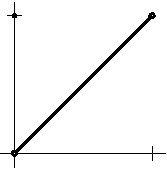
\includegraphics{../figures/limvaldiff}
\end{center}

\pause

\textbf{Proof:}  Let $\epsilon > 0$ be given.

\pause
Let $\delta \coloneqq \epsilon$.

\pause
For $x \in [0,1)$, $x \not= 0$, and $\abs{x-0} < \delta$, we get
\quad
$\abs{f(x) - 0} = \abs{x} < \delta = \epsilon$.
\qed

\end{frame}

\begin{frame}
\begin{lemma}
Let $S \subset \R$, let $c$ be a cluster point of $S$, let $f \colon S \to
\R$ be a function, and let $L \in \R$.

\pause
Then
$f(x) \to L$ as $x \to c$ if and only if for every sequence
$\{ x_n \}_{n=1}^\infty$ in
$S \setminus \{c\}$
such that $\lim\limits_{n\to\infty} x_n = c$,
we have that the sequence $\{ f(x_n) \}_{n=1}^\infty$ converges to $L$.
\end{lemma}

\pause
\textbf{Proof:}
Suppose $f(x) \to L$ as $x \to c$, and $\{ x_n \}_{n=1}^\infty$ is a seq. in
$S \setminus \{c\}$ and $\lim\limits_{n\to\infty} x_n = c$.

\pause
Let $\epsilon > 0$ be given.

\pause
Find $\delta > 0$ such that
if $x \in S \setminus \{c\}$ and $\abs{x-c} < \delta$, then
$\abs{f(x) - L} < \epsilon$.

\pause
Find an $M$ such that for $n \geq M$, we have $\abs{x_n - c} < \delta$.

\pause
\thus \quad for $n \geq M$, \quad
$\abs{f(x_n) - L} < \epsilon$
\pause
\wthus $\{ f(x_n) \}_{n=1}^\infty$ converges to $L$.

\pause
\medskip

Now suppose
it is not true that $f(x) \to L$ as $x \to c$.

\pause
(i.e., $\exists \epsilon > 0 ~ \text{s.t.} \forall \delta > 0 ~ \exists x \in S
\setminus \{ c \}$ where $\abs{x-c} < \delta$ and $\abs{f(x)-L} \geq
\epsilon$.)

\pause
\thus \quad 
$\exists$ $\epsilon > 0$ s.t. $\forall$ $n \in \N$,
$\exists$ $x_n \in S \setminus \{c\}$, where
$\abs{x_n-c} < \nicefrac{1}{n}$ and $\abs{f(x_n)-L} \geq \epsilon$.

\pause
$\{ x_n \}_{n=1}^\infty$ converges to $c$, but
$\{ f(x_n) \}_{n=1}^\infty$ does not converge to $L$.
\qed

\pause
\medskip

\textbf{Exercise:} It is possible to strengthen the $\Leftarrow$:
It is enough to suppose that
$\{ f(x_n) \}_{n=1}^\infty$ converges for every $\{ x_n \}_{n=1}^\infty$ without requiring a specific limit.
\end{frame}

\begin{frame}

\textbf{Example:}
$\displaystyle \lim_{x \to 0} \, \sin( \nicefrac{1}{x} )$
does not exist, but 
$\displaystyle \lim_{x \to 0} \, x\sin( \nicefrac{1}{x} ) = 0$.

\pause
\medskip

Graphs of $\sin(\nicefrac{1}{x})$ and $x \sin(\nicefrac{1}{x})$:

\medskip

\resizebox{4.5in}{1.0in}{\subimport*{../figures/}{sin1x_xsin1x.pdf_t}}

\pause
\medskip

\textbf{Proof:}
Define
$x_n \coloneqq \frac{1}{\pi n + \nicefrac{\pi}{2}}$, so that $x_n \to 0$
\pause
\wthus $\sin ( \nicefrac{1}{x_n} )
\pause
=
\sin (\pi n + \nicefrac{\pi}{2})
\pause
= {(-1)}^n$

\pause
\thus \quad $\bigl\{ \sin ( \nicefrac{1}{x_n} ) \bigr\}_{n=1}^\infty$ does not converge
\pause
\wthus
$\displaystyle \lim_{x \to 0} \, \sin( \nicefrac{1}{x} )$ does not exist.

\pause
\medskip

Let $\{ x_n \}_{n=1}^\infty$ a sequence in $\R \setminus \{ 0 \}$ such that
$\lim\limits_{n\to\infty} x_n = 0$.

\pause
$\abs{\sin(t)} \leq 1$ for all $t \in \R$
\pause
\quad \thus \quad
$
\abs{x_n\sin(\nicefrac{1}{x_n})-0}
=
\abs{x_n}\abs{\sin(\nicefrac{1}{x_n})}
\pause
\leq
\abs{x_n}$.

\pause
\medskip

$x_n \to 0$
\pause
\wthus
$\abs{x_n} \to 0$
\pause
\wthus
$x_n\sin(\nicefrac{1}{x_n}) \to 0$
\pause
\wthus
$\displaystyle \lim_{x \to 0} \, x\sin( \nicefrac{1}{x} ) = 0$.
\qed

\pause
\medskip

\textbf{Remark:} Keep
in mind the ``for every sequence'':

\pause
If $x_n \coloneqq \nicefrac{1}{\pi n}$, then
$\{ \sin (\nicefrac{1}{x_n}) \}_{n=1}^\infty = \{ 0 \}_{n=1}^\infty$, but $\displaystyle \lim_{x\to 0}
\sin(\nicefrac{1}{x})$ DNE.
\end{frame}

\begin{frame}

\begin{corollary}
Let $S \subset \R$ and let $c$ be a cluster point of $S$.  
Suppose $f \colon S \to
\R$ and $g \colon S \to \R$ are functions
such that
the limits of $f(x)$ and $g(x)$ as $x$ goes to $c$ both exist,
and
\begin{equation*}
f(x) \leq g(x) \qquad \text{for all } x \in S \setminus \{ c \}.
\end{equation*}
\pause
Then
\begin{equation*}
\lim_{x\to c} f(x) \leq \lim_{x\to c} g(x) .
\end{equation*}
\end{corollary}

\pause
\textbf{Proof:}
Take $\{ x_n \}_{n=1}^\infty$ be a sequence in $S \setminus \{ c \}$
converging to $c$.

\pause
\medskip

Let \quad
$\displaystyle L_1 \coloneqq \lim_{x\to c} f(x)$
\quad and \quad
$\displaystyle L_2 \coloneqq \lim_{x\to c} g(x)$.

\pause
\medskip

By the lemma above,
$\{ f(x_n) \}_{n=1}^\infty$ converges to $L_1$ and
$\{ g(x_n) \}_{n=1}^\infty$ converges to $L_2$.

\pause
\medskip

We also have $f(x_n) \leq g(x_n)$ for all $n \in \N$.

\pause
\medskip

\thus \quad $L_1 \leq L_2$ ~(by lemma about sequence limits)
\qed
\end{frame}

\begin{frame}

Proofs of the next corollaries are exercises.

\pause
\begin{corollary}
Let $S \subset \R$ and let $c$ be a cluster point of $S$.  Suppose $f \colon S \to
\R$ is such that the limit of $f(x)$ as $x \to c$ exists.
Suppose $\exists$ $a,b \in \R$ such that
~$a \leq f(x) \leq b$ for all $x \in S \setminus \{ c \}$.

\pause
\medskip

Then \quad $\displaystyle a \leq \lim_{x\to c} f(x) \leq b$.
\end{corollary}

\pause
\begin{corollary}
Let $S \subset \R$ and let $c$ be a cluster point of $S$.
Suppose $f \colon S \to \R$,
$g \colon S \to \R$, and $h \colon S \to \R$ are such that
~~$f(x) \leq g(x) \leq h(x)$ for all $x \in S \setminus \{ c \}$.

\pause
\medskip

Suppose $\displaystyle \lim_{x\to c} f(x) = \lim_{x\to c} h(x)$
~~(in particular, the limits exist).

\pause
\medskip

Then the limit of $g(x)$ as $x$ goes to $c$ exists and
~~$\displaystyle \lim_{x\to c} g(x) =
\lim_{x\to c} f(x) = \lim_{x\to c} h(x)$.
\end{corollary}

\end{frame}

\begin{frame}

\begin{corollary}
Let $S \subset \R$ and let $c$ be a cluster point of $S$.  
Suppose $f \colon S \to \R$ and
$g \colon S \to \R$ are 
such that 
the limits of $f(x)$ and $g(x)$ as $x$ goes to $c$ both exist.
\pause
Then
\begin{enumerate}[(i)]
\item
$\displaystyle
\lim_{x\to c} \bigl(f(x)+g(x)\bigr) = \left(\lim_{x\to c} f(x)\right) + 
\left(\lim_{x\to c} g(x)\right) .
$
\item
\pause
$\displaystyle
\lim_{x\to c} \bigl(f(x)-g(x)\bigr) = \left(\lim_{x\to c} f(x)\right) -
\left(\lim_{x\to c} g(x)\right) .
$
\item
\pause
$\displaystyle
\lim_{x\to c} \bigl(f(x)g(x)\bigr) = \left(\lim_{x\to c} f(x)\right)
\left(\lim_{x\to c} g(x)\right) .
$
\item\pause\label{falg:cor:iv}
If
$\displaystyle \lim_{x\to c} g(x) \not= 0$,
and $g(x) \not= 0$ for all $x \in S \setminus \{ c \}$, then
$\displaystyle
\lim_{x\to c} \frac{f(x)}{g(x)} =
\frac{\lim_{x\to c} f(x)}{\lim_{x\to c} g(x)}$.
\end{enumerate}
\end{corollary}

\pause
\begin{corollary}
Let $S \subset \R$ and let $c$ be a cluster point of $S$.
Suppose $f \colon S \to \R$ is such that $\lim\limits_{x\to c} f(x)$ exists.

\pause
\medskip

Then
\quad
$\displaystyle
\lim_{x\to c} \abs{f(x)} =
\abs{\lim_{x\to c} f(x)}$.
\end{corollary}

\end{frame}

\begin{frame}

\begin{definition}
Let $f \colon S \to \R$ be a function and $A \subset S$.  Define the
function $f|_A \colon A \to \R$ by
\begin{equation*}
f|_A (x) \coloneqq f(x)  \qquad \text{for } x \in A.
\end{equation*}
\pause
The function
$f|_A$ is called the \emph{restriction} of $f$ to $A$.
\end{definition}

\pause
The function $f|_A$ is simply the function $f$ taken on a smaller domain.

\pause
\medskip

Be careful, e.g., $f \colon \R \to \R$ defined by say $f(x) \coloneqq x^2$

and $f|_{[0,1]} \colon [0,1] \to \R$ really are different functions.

\pause
\medskip

E.g., it is \textbf{not} true that $f|_{[0,1]}(2) = 2^2$.
\pause {\color{red} \hspace*{-0.9in} XXXXXXXX~~}
\quad $f|_{[0,1]}(2)$ is
\textbf{not defined}. \quad But $f(2)=2^2$

\end{frame}

\begin{frame}

\begin{proposition}
Let $S \subset \R$, $c \in \R$, and
let $f \colon S
\to \R$ be a function.
\pause
Suppose
$A \subset S$ is such that there is some $\alpha > 0$ such that
$(A \setminus \{ c \}) \cap (c-\alpha,c+\alpha) = (S \setminus \{ c \}) \cap (c-\alpha,c+\alpha)$.
\pause
\begin{enumerate}[(i)]
\item
The point $c$ is a cluster point of $A$ if and only if $c$ is a cluster point
of $S$.
\item\pause
Let $c$ be a cluster point of $S$. ~ $f(x) \to L$ as $x \to c$
\wiffif
$f|_A(x) \to L$ as $x \to c$.
\end{enumerate}
\end{proposition}

\pause
\textbf{Proof:}
First, let $c$ be a cluster point of $A$, and note that $A \subset S$.

\pause
$( A \setminus \{ c\} ) \cap (c-\epsilon,c+\epsilon) \not= \emptyset$
~$\forall$ $\epsilon > 0$
\pause
\wthus
$( S \setminus \{ c\} ) \cap
(c-\epsilon,c+\epsilon) \not= \emptyset$
~$\forall$ $\epsilon > 0$.

\pause
\thus \quad $c$ is a cluster point of $S$.

\pause
\medskip

Second, suppose $c$ is a cluster point of $S$.

\pause
For $\epsilon > 0$ s.t.  $\epsilon < \alpha$, we get $( A \setminus \{ c\} ) \cap (c-\epsilon,c+\epsilon) =
( S \setminus \{ c\} ) \cap (c-\epsilon,c+\epsilon) \not= \emptyset$.

\pause
As it is true for all $\epsilon < \alpha$,
\quad
$( A \setminus \{ c\} ) \cap (c-\epsilon,c+\epsilon) \not=\emptyset$ for all
$\epsilon > 0$.

\pause
\thus \quad $c$ is a cluster point of $A$.

\end{frame}

\begin{frame}

Suppose $c$ is a cluster point of $S$ and therefore also a cluster point of $A$.

\pause
\medskip

Suppose $f(x) \to L$ as $x \to c$:

\pause
$\forall$ $\epsilon > 0$ ~ $\exists$ $\delta > 0$ such that if $x \in S \setminus \{ c \}$
and $\abs{x-c} < \delta$, then $\abs{f(x)-L} < \epsilon$.

\pause
If $x \in A \setminus \{ c \}$, then $x \in S \setminus \{ c \}$.

\pause
\thus \quad $f|_A(x) \to L$ as $x \to c$.

\pause
\medskip

Finally, suppose $f|_A(x) \to L$ as $x \to c$ and let $\epsilon > 0$ be
given.

\pause
$\exists$ $\delta' > 0$ such that if $x \in A \setminus \{ c \}$
and $\abs{x-c} < \delta'$, then $\bigl\lvert f|_A(x)-L \bigr\rvert < \epsilon$.

\pause
Take $\delta \coloneqq \min \{ \delta', \alpha \}$.

\pause
Suppose $x \in S \setminus \{ c \}$ and
$\abs{x-c} < \delta$.

\pause
$\abs{x-c} < \alpha$ \wthus $x \in A \setminus \{ c \}$,

\pause
$\abs{x-c} < \delta'$ \wthus $\abs{f(x)-L} = \bigl\lvert f|_A(x)-L \bigr\rvert < \epsilon$.
\qed

\pause
\medskip

\textbf{Remark:}
The hypothesis on $A$ in the proposition is necessary.

\pause
Without it, we only get one implication (exercise):

\pause
Assume $c$ is a cluster point of $A$, then

$f(x) \to L$ as $x \to c$
\wthus
$f|_A(x) \to L$ as $x \to c$.

\pause
\medskip

\textbf{Notation:}
\quad $\displaystyle
\lim_{\substack{x \to c\\x \in A}} f(x) \coloneqq \lim_{x \to c} f|_A(x)$.

\end{frame}

\begin{frame}

\begin{definition}[One sided limits]
Let $f \colon S \to \R$ be function and $c \in \R$.

\pause
\medskip

If $c$ is a cluster point of $S \cap (c,\infty)$ and the limit
of $f|_{S \cap (c,\infty)}$ 
as $x \to c$ exists, define
\begin{equation*}
\lim_{x \to c^+} f(x) \coloneqq \lim_{x\to c} f|_{S \cap (c,\infty)}(x) .
\end{equation*}

\pause
If $c$ is a cluster point of 
$S \cap (-\infty,c)$ and the limit
of $f|_{S \cap (-\infty,c)}$ 
as $x \to c$ exists, define
\begin{equation*}
\lim_{x \to c^-} f(x) \coloneqq \lim_{x\to c} f|_{S \cap (-\infty,c)}(x) .
\end{equation*}
\end{definition}

\pause
Many common notations: 

\medskip

For
~$\lim\limits_{x \to c^-} f(x)$~ one sees
~$\lim\limits_{\substack{x \to c\\x < c}} f(x)$,~
~$\lim\limits_{x \uparrow c} f(x)$,~ or
~$\lim\limits_{x \nearrow c} f(x)$.

\medskip

For
~$\lim\limits_{x \to c^+} f(x)$~ one sees
~$\lim\limits_{\substack{x \to c\\x > c}} f(x)$,~
~$\lim\limits_{x \downarrow c} f(x)$,~ or
~$\lim\limits_{x \searrow c} f(x)$.


\end{frame}

\begin{frame}

The proposition above does not apply to one-sided limits.

\pause
\medskip

\textbf{Example:}
Define $f \colon \R \to \R$ by $f(x) \coloneqq 1$ for $x < 0$ and
$f(x) \coloneqq 0$ for $x \geq 0$. Then
\begin{equation*}
\lim_{x \to 0^-} f(x) = 1, \qquad
\lim_{x \to 0^+} f(x) = 0, \qquad
\lim_{x \to 0} f(x) \quad \text{does not exist.}
\end{equation*}

\pause
\medskip

But we do have:

\begin{proposition}
Let $S \subset \R$ be such that $c$ is a cluster point
of both $S \cap (-\infty,c)$ and $S \cap (c,\infty)$, let
$f \colon S \to \R$ be a function, and let $L \in \R$.
\pause
Then $c$ is a cluster point of $S$ and
\begin{equation*}
\lim_{x \to c} f(x) = L
\qquad \text{if and only if} \qquad
\lim_{x \to c^-} f(x) =
\lim_{x \to c^+} f(x) =
L .
\end{equation*}
\end{proposition}

\pause
\textbf{Proof:} Exercise.

\pause
\medskip

Hint:
$\bigl( S \cap (-\infty,c) \bigr) \cup \bigl( S \cap (c,\infty) \bigr)
= S \setminus \{ c \}$.
\end{frame}

\begin{frame}
Composition also plays nice with limits if one is careful:

\pause
\medskip

\textbf{Exercise:}
Let $c_1$ be a cluster point of $A \subset \R$ and $c_2$ be a cluster point of $B \subset \R$.

\pause
Suppose $f \colon A \to B$ and $g \colon B \to \R$ are
such that $f(x) \to c_2$ as $x \to c_1$ and
$g(y) \to L$ as $y \to c_2$.

\pause
If $c_2 \in B$, also suppose that $g(c_2) = L$ (important).

\pause
Let $h(x) \coloneqq g\bigl(f(x)\bigr)$.  Show
$h(x) \to L$ as $x \to c_1$.

\pause
\medskip

Hint: Note that $f(x)$ could equal $c_2$ for many $x \in A$.
\end{frame}

\end{document}
